\section{Implementation}

\begin{figure}[htbp]
 \centering
 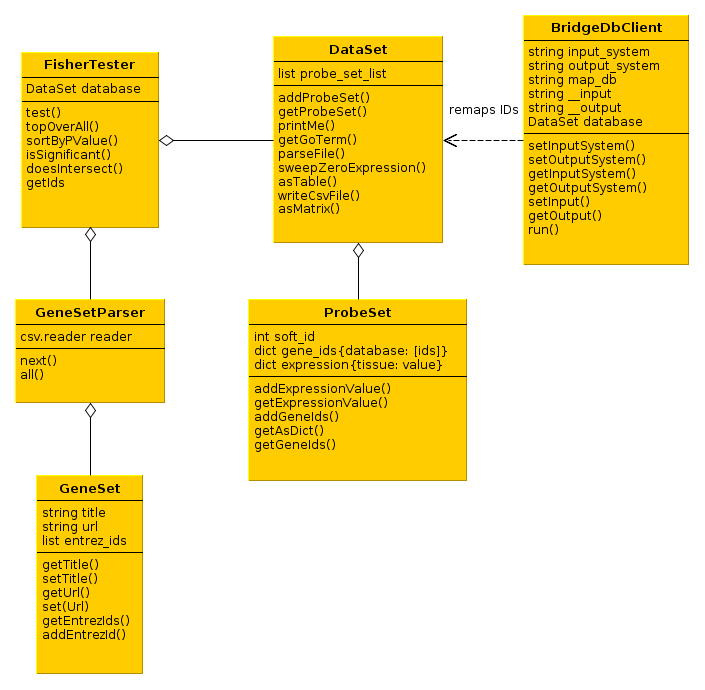
\includegraphics[scale=0.5]{../pibi_uml.png}
 % pibi_uml.png: 919x496 pixel, 72dpi, 32.42x17.50 cm, bb=0 0 919 496
 \caption{UML scheme}
 \label{fig:uml}
\end{figure}


  \subsection[SVN Repository]{Subversion Repository}
  Python source code for all implemented scripts, UML schemata and the
documentation (including this report) is hosted at
\url{https://xp-dev.com/svn/pibi} using the Subversion (SVN) version control
system.
  
  \subsection[Geo SOFT parser]{Geo SOFT parser for Affymetrix MicroArray data}
  
  The classes ProbeSet and DataSet were designed to represent the expression
values from an Affymetrix Human Exon 1.0 ST Array as used in \cite{Berger2010}.
The experiment-specific SOFT ID for each probeset serves as unique key or
identifier for instances of the ProbeSet class, which also have a dictionary of
gene identifiers by database and a dictionary of expression values by tissue as
attributes. An instance of a DataSet is composed of a list of ProbeSets. Instead
of the suggested GEO parser included in the Bio package we use our own parser to
read the SOFT file obtained from
\url{http://www.ncbi.nlm.nih.gov/geo/query/acc.cgi?acc=GSE17593}.
  
  The parser method \lstinline|parseFile()| processes a Geo SOFT file (eg.
GSE17593\_family.soft from aforementioned experiment) by first scanning the
platform section of the Affymetrix array (identified by the ID code ``GPL5175``)
for Ensemble and NCBI gene IDs associated with each SOFT ID and adding them to
the corresponding dictionaries. The parser then proceeds to the sample section
and reads all expression values from samples that were present on the Affymetrix
array, thus excluding any GenomeAnalyzer II RNAseq and SNP array data.
  
  In a final step, the method \lstinline|sweepZeroExpression()| is called to
remove all ProbeSets from the DataSet that do not contain expression values -
these entries were created in the initial parsing step of the platform table but
not populated in the second step. The resulting list of ProbeSets contains 17381
entries, matching the expected number of unique Affymetrix Human Exon 1.0 ST
Array probesets that are included in the original SOFT file.
  
  \subsection[BridgeDB wrapper]{Wrapping of BridgeDB for translation and aggregation of gene IDs}
  
  The translation of Ensembl IDs to gene identifiers used in other repositories
for genetic information like Entrez, UniProt and Gene Ontology requires access
to the ID mapping framework like BridgeDb (\url{http://www.bridgedb.org/}),
which is available as a local web service within the WSI network
(\url{http://pride:8183}) and can be queried through HTTP \lstinline|GET|
requests to specific URIs as listed and explained at
\url{http://www.bridgedb.org/wiki/BridgeWebservice}. As repeated HTTP requests
for all IDs in the DataSet would likely fail due to network latency we use
\lstinline|batchmapper.sh|, a scripted version of BridgeDb available at
\lstinline|/share/opt/noarc/BridgeDB/bridgedb-1.1.0/batchmapper.sh|, to speed up
the ID mapping process. The class \lstinline|BridgeDbClient| has attributes for
all parameters of the script and wraps its functionality in the
\lstinline|remap()| method by setting the input system code (EnHs = Ensembl Homo
sapiens), the output system code (L = Entrez, S = UniProt or T = GeneOntology
ID), the path to an Apache Derby database containing the mappings
(\lstinline|/share/data/bridgedb/Hs_Derby_20110601.bridge|) and calling the
shell script via \lstinline|os.system()| in the \lstinline|run()| method. The
temporary output file created by the script is then parsed by
\lstinline|getOutput()| and either directly appended to the DataSet (if provided
as input) or returned as list.

  \subsection[GO terms]{Retrieval of GO terms using goatools}
  
  With GO IDs now being available in the DataSet a method to also query the
corresponding GO term descriptions is needed. We use the \lstinline|goatools|
module available at \url{https://github.com/tanghaibao/goatools/} to parse the
OBO flat file format that stores all GO IDs and their descriptions (see
\url{http://www.geneontology.org/GO.format.obo-1_2.shtml} for the v1.2
specification). A call of \lstinline|getGoTerm()| on a DataSet instance passes
the queried GO ID to the method \lstinline|query_term| of a \lstinline|GODag|
instance working on a recent Gene Ontology OBO flat file (downloaded from
\url{http://www.geneontology.org/ontology/obo_format_1_2/gene_ontology.1_2.obo})
and returns the GO term desciption as output string.

  \subsection[Heatmap]{Visualization of expression values as heatmap}
  
  A heatmap of expression values was created using the R script
\lstinline|heatmap.R| provided by the tutors. It reads the CSV output of a
DataSet (specifically columns 8 to 16, which contain the expression values by
tissue sample) in line 1, determines the mean expression value of each probeset
over all nine tissues (line 2) as well as the maximum deviation from the mean
per probeset row (line 3), then filters out samples with less than 1.0 deviation
from the mean (remaining probesets are at least twofold over- or underexpressed
compared to the mean) in line 4. The \lstinline|apply()| function in line 5
first centers all filtered probesets by subtracting the means over all tissue
columns from the individual expression values and then scaled by dividing them
by their standard deviations (see
\url{http://stat.ethz.ch/R-manual/R-devel/library/base/html/scale.html}). Lines
6 to 8 then create a JPEG file of the output of \lstinline|heatmap()|, which
produces a false-color representation of expression value z-scores on a
yellow-red scale with additional dendrograms of distances on both the sample and
the probeset axis.

\lstset{language=R}
\begin{lstlisting}  
d <-read.table("../data_out.csv", header=T, sep=",")
d_mean <- rowMeans(d[,8:16])
d_maxfc <- apply(d[,8:16],1,function(x) max(max(x)-mean(x), abs(min(x)-mean(x))))
d_filtered <- d[which(d_maxfc > 1.0),]
d_filtered_z <- apply(d_filtered[,8:16],1,scale)
jpeg('heatmap.jpg')
heatmap(d_filtered_z)
dev.off()
\end{lstlisting}
  
  \subsection[z-scores and p-values]{Calculation of z-scores and p-values}
      
  The z-score is calculated as follows:
  \begin{equation}
  z=\frac{x-\mu}{\sigma}
  \end{equation}
  where $\mu$ is the expected value and $\sigma$ the standard deviation. An
important distinction is whether to take the mean and deviation from the columns
or the rows. In our case, columns stand for different tissues, rows for
different genes. Therefore we used the mean and standard deviation for each row
in order to compare the tissues regarding a certain gene.
  
  In our implementation we calculated the p-values upon the z-scores obtained
from the expression levels. For computation we used the scipy function \lstinline|ndtr()|
which returns the area under the standard Gaussian probability density function
starting from a point $x$ to infinity. We used a two-sided p-value, therefore
the final function call was as follows:
  \lstset{language=Python}
\begin{lstlisting}
2 * special.ndtr(numpy.absolute(z_score) * -1)
\end{lstlisting}
  
  \subsection[GMT file parsing]{Parsing GMT file for gene sets}
  
  GMT are text-based files that contain one geneset per row. Each tab-delimited
row has a geneset title string, a URL pointing to metadata on the geneset and a
list of comma-separated Entrez IDs. The structure of these data was modeled in a
basic \lstinline|GeneSet| class with three attributes and the corresponding
\lstinline|get| and \lstinline|set| methods. The class \lstinline|GeneSetParser|
is responsible for reading the passed GMT file and returning GeneSet entities -
either individually or as list. As the GMT format is basically a CSV format with
tab instead of comma delimiters the GeneSetParser simply wraps the
\lstinline|csv.reader()| class and \lstinline|next()| method and splits the row
items into title, URL and Entrez IDs. An additional \lstinline|all()| method
returns a list of all GeneSet instances when called.
  
  \subsection[Gene set enrichment]{Gene set enrichment}
    \subsubsection[Fisher exact test]{Fisher exact test}
    As described in section \ref{sec:fisher}, the fisher's exact test is based
on contingency tables. Therefore we implemented a method counting every
significant gene ($\text{p-value} < 0.05$) for every tissue contained in a gene
set. The contingency table is structured as follows:
\begin{center}
$\left[\begin{array}{cc}
\text{significant \& in geneset} & \text{significant \& not in geneset} \\
\text{not significant \& in geneset} & \text{not significant \& not in geneset} \\
\end{array}\right]$
\end{center}
    Each cell contains the gene count for a combination of gene set and tissue
    with the specified characteristics.

    For every contingency table a fisher's exact test was computed using the
scipy implementation. As scoring measure we used the p-value received from the
test. As result we received a list of all gene sets for every tissue with an
attached p-value, indicating if the geneset is significantly up- or down
regulated within the current tissue.
    
    \subsubsection[GSEA]{GSEA}
    For GSEA we used pure expression levels as provided in the dataset as GSEA
will perform standardizing methods by its own (see \cite{Subramanian2005} for
details) For output we had to filter out those genes with no matching Entrez
IDs, as GSEA matches those IDs to genesets. Furthermore GSEA filters out those
genesets which have less then 15 or more then 500 hits within our data. All
settings were left at their default values. As we did not have control
groups, every tissue has been tested against all others, resulting in 18
different runs. HTML output and shows relevant plots were automatically created
by GSEA.